%&pdflatex
\documentclass{standalone}
%\documentclass[a4paper, landscape]{article}
\usepackage{graphicx}
\usepackage{pbox}

\newcommand{\picHeight}{1in}
\begin{document}

        \begin{tabular}{| c | c | c | c | c |}
            \hline
            \pbox{20cm}{Config-\\uration} &
            %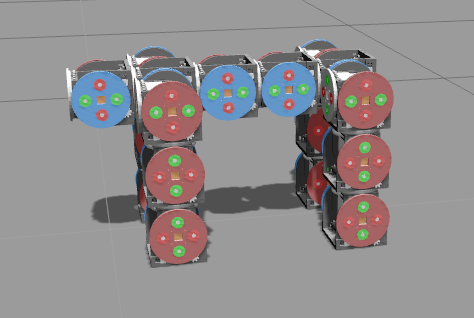
\includegraphics[height=\picHeight]{walk4.png} &
            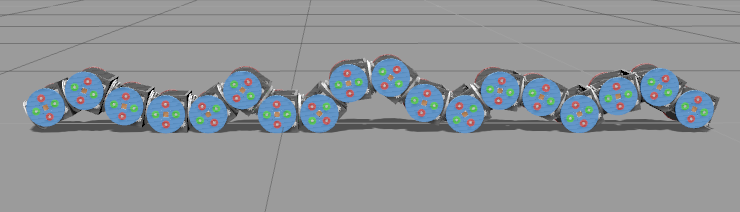
\includegraphics[width=4cm]{snake18.png} &
            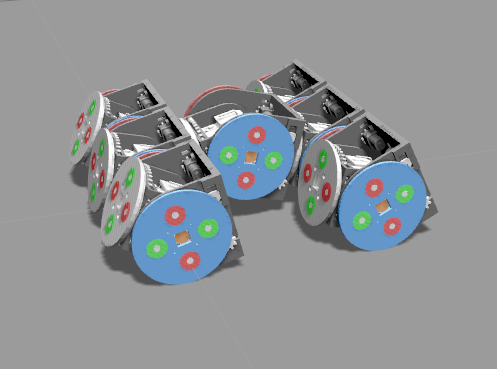
\includegraphics[height=\picHeight]{car.png} &
            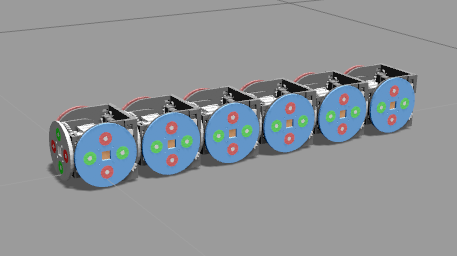
\includegraphics[width=4cm]{../body.png} 
             \\ 
            ~ & %WALK4 & C
            CHAIN18 & CAR & CHAIN6 \\ \hline
            \pbox{20cm}{Compo-\\nents} &
            %\pbox{20cm}{BODY3 \\ LEG3 \(\times4\)} &
            \pbox{20cm}{CHAIN3 \(\times6\)} &
            \pbox{20cm}{CHAIN3 \\ MODULE \(\times4\)} &
            \pbox{20cm}{CHAIN3 \(\times2\)}
            \\ \hline
            \pbox{20cm}{Beha-\\viors} &
            %\pbox{20cm}{\(Walk(t)\)} &
            \pbox{20cm}{\(SineGait18()\)} &
            \pbox{20cm}{\(Drive(v,t)\) \\ \(Turn(\theta)\)} &
            \pbox{20cm}{\(Drive(v,t)\), \(Turn(\theta)\) \\ \(HoldRigid()\) }
            \\ \hline
        \end{tabular}
\end{document}








